
\documentclass[10pt,letterpaper]{article}

\usepackage{hyperref}
\usepackage{cogsci}
\usepackage{pslatex}
\usepackage{pdfsync}
\usepackage{amsmath}
\usepackage{graphicx}
\usepackage{topcapt}
\usepackage{color}


\title{Large scale investigations of variability in early language production}
\author{{\large \bf Rose M. Schneider} \\ \texttt{rschneid@stanford.edu}\\ Department of Psychology \\ Stanford University \\ 
\And {\large \bf Dan Yurovsky} \\ \texttt{yurovsky@stanford.edu} \\ Department of Psychology \\ Stanford University \\ 
\And {\large \bf Michael C. Frank} \\ \texttt{mcfrank@stanford.edu} \\ Department of Psychology \\ Stanford University \\ }

\begin{document}
\maketitle


%ABSTRACT
\begin{abstract}
The first word, an intimate moment between child and caretaker, exhibits a tremendous amount of variability in semantic categorization, phonological complexity, and age of onset. Through several large datasets of parental report of children’s first words, we investigate patterns in first word production, including the age of onset, distribution of MB-CDI categories, and first words in relation to parental input. In three analyses, we explore the timecourse and distribution of children’s first recognizable language productions. We find that, contra conventional wisdom, more than 75% of children in our datasets produce a first word by their first birthday. In our second analysis, we find that older children produce more words in certain semantic categories. Finally, we take all the unique occurrences of words across the datasets, and try to predict first word production via parental input taken from the CHILDES corpus. Overall, we find that parental report of a child’s first word yields rich and consistent data on what is typically an unobservable dyadic moment, and that the words children produce first may be affected by semantic differences as well as by parental input.

\textbf{Keywords:}
language acquisition
\end{abstract}

%%INTRODUCTION%%%%
\section{Introduction}
- The emergence of language is cool
- Paragraph - first word comprehension - Bergelson and Swingley
- Paragraph - Why are we interested in first productions?
- Paragraph - parent report - advantages and drawbacks 
- Paragraph - summary of our work

%%GENERAL DATA METHODS%%
\section{General Data Collection Methods}
Data for this study is comprised of 4 different datasets, each obtained from a different source. Three of the 4 datasets were drawn from surveys specifically designed for this study. The last dataset contains data from Wordbank, an online repository of data from the MacArthur-Bates Communicative Development Inventories, a widely-used parent-report vocabulary checklist (Fenson et al., 2007). 

%CDM
\section{Dataset 1: Children's Discovery Museum Survey}

\subsection{Participants}
We sent out a brief survey on children’s first words to subscribed members of a large local children’s museum. We received 502 responses to our survey (215 female, 285 male, and 2 with no reported gender; M age = 11 mo, median = 10 mo). Due to the diversity of the San Jose community, several of the first word responses were not in English. Responses were translated into English where possible. Responses that were not able to be translated were excluded from further analysis (N = 1).

\subsection{Methods}
Parents completed a brief web-based survey (created with JavaScript and HTML). The survey asked parents to list their child’s first word (excluding “mama” and “dada”), what they thought word referred to, a description of the situation surrounding the first word, the child’s age at time of utterance (≤10 mo or younger, 11 mo, 12 mo, 13 mo, ≥14 mo), the child’s current age, and their gender. Parents answered for only one child in this survey.

\subsection{Data preparation}
Parents’ responses were standardized for ease of analysis. Data cleaning involved fixing obvious spelling errors. When the meaning of the word was not immediately apparent, the researcher relied on the parent’s description of the circumstances surrounding the word and/or the parent’s classification of the word type.

%SURVEY2
\section{Dataset 2: Amazon Mechanical Turk}

\subsection{Participants}
We recruited 1000 parents from Amazon Mechanical Turk to complete an updated survey on their children’s first words. We restricted the survey to parents in the United States. This survey allowed parents to answer for multiple children. We received 1671 responses (813 female, 858 male; M age = 10 mo, median = 10 mo). 21 children were excluded from subsequent analyses because they had not yet spoken (M age = 2.7 mo, median = 2 mo). Responses were translated into English when possible and required. Responses that were not able to be translated were excluded from further analysis (N = 1).

\subsection{Methods}s
This survey was an extended version of the previous one. They survey allowed for input for multiple children, and asked parents to list their highest education level, child's birth order, sex,  first word (excluding “mama” and “dada”), word type, addressee of the first word, word age (0 – 24+ months), current age (0 – 18+ years), word language, and home language.  Responses were validated as the survey was completed, reducing the likelihood of erroneous or false responses. 

\subsection{Data preparation}
Data were handled as in Dataset 1. Due to the larger sample size, more phonological and morphological variations appeared. A final standardized form was selected, and the various original first word forms became that standardized form. For example,  “Dog dog”, “Doggy”, “Doggie”, and “Dogie” were all treated as “Dog” in the standardized form. We occasionally had to rely on the parent’s description of the situation of the word occurrence to inform our decisions.

%%%SURVEY 3
\section{Dataset 3: Contemporary Psycholinguist Diary Studies}

\subsection{Participants}
We sent out a brief survey on children's first words to subscribed members of a Psycholinguist listserv. We received 52 responses from this survey (26 female, 26 male; M age = 11.16 mo, median 11 mo).

\subsection{Methods}
Questions included on the survey were: The approximate phonological form of the  first word, the age of the utterance, when the parent recorded this (if at all), the child’s sex, the target word, the child’s birth order (first or later born), and the child’s current age. 

 \subsection{Data processing}
Data were handled similarly to Datasets 1 and 2. 

%%%%WORDBANK%%%%
\section{Dataset 4: MB-CDI Wordbank}

\subsection{Participants}

\subsection{Methods}

\subsection{Data preparation}

%Analyses
\subsection{Age} 
Conventional wisdom generally cites 12 months as the harbinger of the first word (Citation here). However, a child's first word is almost exclusively heard by a parent or other caretaker, and next to impossible to capture in a lab setting. However, that milestone is subject to the extreme variability in early language production (Fenson, 1994) and the potential pitfalls of parental memory (as discussed above). Given the possibility of very early noun comprehension (Bergelson and Swingley), we wished to explore the development of first word production, especially prior to 12 months. If children consistently produce a word-like utterance before 12 months, it is possible that very early language production does happen, but potentially in a phonologically unrecognizable and inconsistent form. \par
Across the 4 datasets, we grouped data (N = 3173) by age and by dataset. Twenty-one children were excluded for not having spoken yet (M age  = 2.7 mo, median = 2 mo). 

%FIGURE 1
\begin{figure}[t]
\begin{center}
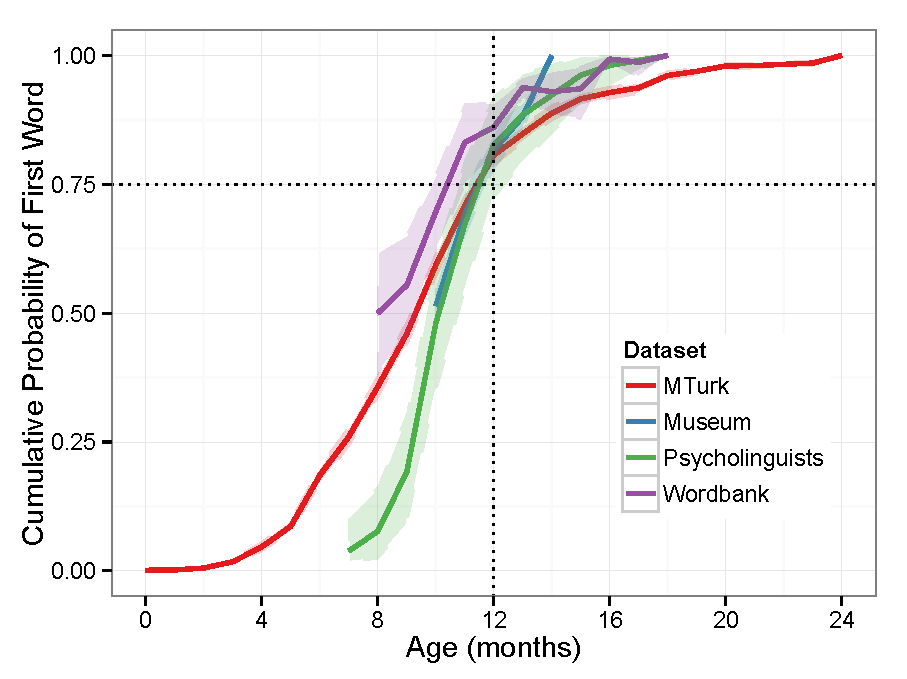
\includegraphics[width=1\linewidth]{Figure1.pdf}
\end{center}
\caption{Figure 1: Age graph showing the cumulative probability of producing a word as a function of age.}\
\end{figure}

- Details of stats
- Differences across studies
- Data suggests

\subsection{CDI Categories} 
- Question
- Describe analyses
- Details of stats
- Differences across studies
- Data suggests

\subsection{Input Frequencies}
- Question
- Describe analyses
- Details of stats
- Differences across studies
- Data suggests

\section{Discussion}

\section{Acknowledgements}




\end{document}
